\documentclass{beamer}

% Theme choice:
\usetheme{Madrid}
\usepackage{setspace}
\usepackage{amssymb}
\usepackage{amsmath}
\usepackage{amsthm}
\usepackage{mathrsfs}
\usepackage{mathtools}
\usepackage{longtable}
\usepackage{graphicx}

\usepackage{listings}
    \usepackage{color}                                            %%
    \usepackage{array}                                            %%
    \usepackage{longtable}                                        %%
    \usepackage{calc}                                             %%
    \usepackage{multirow}                                         %%
    \usepackage{hhline}                                           %%
    \usepackage{ifthen}                                           %%
    \usepackage{lscape}     
    \usepackage{amsmath}
\def\inputGnumericTable{}
\newcommand{\mydet}[1]{\ensuremath{\begin{vmatrix}#1\end{vmatrix}}}
\newcommand{\myvec}[1]{\ensuremath{\begin{pmatrix}#1\end{pmatrix}}}
\providecommand{\pr}[1]{\ensuremath{\Pr\left(#1\right)}}
\providecommand{\cbrak}[1]{\ensuremath{\left\{#1\right\}}}
\providecommand{\brak}[1]{\ensuremath{\left(#1\right)}}
\newcommand*{\permcomb}[4][0mu]{{{}^{#3}\mkern#1#2_{#4}}}
\newcommand*{\perm}[1][-3mu]{\permcomb[#1]{P}}
\newcommand*{\comb}[1][-1mu]{\permcomb[#1]{C}}

% Title page details: 
\title{Assignment 7 - Presentation} 
\author{Varshini Jonnala - CS21BTECH11024}
\date{\today}

\begin{document}

% Title page frame
\begin{frame}
    \titlepage 
\end{frame}


% Outline frame
\begin{frame}{Outline}
    \tableofcontents
\end{frame}

\section{Abstract}
\begin{frame}{Abstract}:
\begin{itemize}
    \item This document contains the solution to Question 3.12 in Chapter 3 of Papoulis Book.
\end{itemize}
\end{frame}

\section{Question}
\begin{frame}{Question}:
\begin{itemize}
    \item 3 dice are rolled and the player may bet on anyone of the face values 1,2,3,4,5 and 6. If the player's number appears on 1,2, or all 3 dice, the player receives respectively 1,2 or 3 times his original stake plus his own money back. Determine the expected loss per unit stake for the player.
\end{itemize}
\end{frame}


% Blocks frame
\section{Solution}
\begin{frame}[allowframebreaks]{Solution}
    Let $k$ be the number that player bets on.
    
    Now, Let the random variable $X \in \cbrak{0,1,2,3}$ denote the number of times $k$ appears on the 3 dice.
    \begin{table}[ht!]
        \def\ifundefined#1{\expandafter\ifx\csname#1\endcsname\relax}
\ifundefined{inputGnumericTable}
	\def\gnumericTableEnd{\end{document}}

	\documentclass[12pt%
			  %,landscape%
                    ]{report}
       \usepackage[latin1]{inputenc}
       \usepackage{fullpage}
       \usepackage{color}
       \usepackage{array}
       \usepackage{longtable}
       \usepackage{calc}
       \usepackage{multirow}
       \usepackage{hhline}
       \usepackage{ifthen}
       \usepackage[misc]{ifsym}
	\begin{document}
\else
    \def\gnumericTableEnd{}
\fi
\providecommand{\gnumericmathit}[1]{#1} 
\providecommand{\gnumericPB}[1]%
{\let\gnumericTemp=\\#1\let\\=\gnumericTemp\hspace{0pt}}
 \ifundefined{gnumericTableWidthDefined}
        \newlength{\gnumericTableWidth}
        \newlength{\gnumericTableWidthComplete}
        \newlength{\gnumericMultiRowLength}
        \global\def\gnumericTableWidthDefined{}
 \fi
 \ifthenelse{\isundefined{\languageshorthands}}{}{\languageshorthands{english}}                                                      %%
\providecommand\gnumbox{\makebox[0pt]}                       %%
\setlength{\bigstrutjot}{\jot}
\setlength{\extrarowheight}{\doublerulesep}
\setlongtables

\setlength\gnumericTableWidth{%
	50pt+%
	170pt+%
0pt}
\def\gumericNumCols{4}
\setlength\gnumericTableWidthComplete{\gnumericTableWidth+%
         \tabcolsep*\gumericNumCols*2+\arrayrulewidth*\gumericNumCols}
\ifthenelse{\lengthtest{\gnumericTableWidthComplete > \linewidth}}%
         {\def\gnumericScale{1*\ratio{\linewidth-%
                        \tabcolsep*\gumericNumCols*2-%
                        \arrayrulewidth*\gumericNumCols}%
{\gnumericTableWidth}}}%
{\def\gnumericScale{1}}


\ifthenelse{\isundefined{\gnumericColA}}{\newlength{\gnumericColA}}{}\settowidth{\gnumericColA}{\begin{tabular}{@{}p{50pt*\gnumericScale}@{}}x\end{tabular}}
\ifthenelse{\isundefined{\gnumericColB}}{\newlength{\gnumericColB}}{}\settowidth{\gnumericColB}{\begin{tabular}{@{}p{170pt*\gnumericScale}@{}}x\end{tabular}}

	\begin{center}
\begin{tabular}[c]{%
	b{\gnumericColA}%
	b{\gnumericColB}%
	}

	\hhline{|-|-~}
	 \multicolumn{1}{|p{\gnumericColA}|}%
	{\gnumericPB{\centering}\gnumbox{\textbf{Event}}}
	&\multicolumn{1}{p{\gnumericColB}|}%
	{\gnumericPB{\centering}\gnumbox{\textbf{Description}}}
\\
    \hhline{|--|~}
	 \multicolumn{1}{|p{\gnumericColA}|}%
	{\gnumericPB{\centering}\gnumbox{$X=0$}}
	&\multicolumn{1}{p{\gnumericColB}|}%
	{\gnumericPB{\centering}\gnumbox{Hanif losing the game}}
\\
    \hhline{|--|~}
	 \multicolumn{1}{|p{\gnumericColA}|}%
	{\gnumericPB{\centering}\gnumbox{$X=1$}}
	&\multicolumn{1}{p{\gnumericColB}|}%
	{\gnumericPB{\centering}\gnumbox{Hanif winning the game}}
\\
\hhline{|-|-|~}
\end{tabular}
	\end{center}
	
\ifthenelse{\isundefined{\languageshorthands}}{}{\languageshorthands{\languagename}}
\gnumericTableEnd

        \caption{Description of Events}
	    \label{Tables:Table}
    \end{table}
    Then,
    \begin{align}
        \pr{X = 0} &= \myvec{3\\0} \brak{\frac{1}{6}}^0 \brak{\frac{5}{6}}^3 = \frac{125}{216}\\
        \pr{X = 1} &= \myvec{3\\1} \brak{\frac{1}{6}}^1 \brak{\frac{5}{6}}^2 = \frac{75}{216}\\
        \pr{X = 2} &= \myvec{3\\2} \brak{\frac{1}{6}}^2 \brak{\frac{5}{6}}^1 = \frac{15}{216}\\
        \pr{X = 3} &= \myvec{3\\3} \brak{\frac{1}{6}}^3 \brak{\frac{5}{6}}^0 = \frac{1}{216}
    \end{align}
    
    Given, If the player's number appears on 1, 2, or all 3 dice, the player receives respectively 1, 2, or 3 times his original stake plus his own money back. 
    
    Hence, The Expected gain per unit stake for the player is
    \begin{align}
        &= \sum_{k=1}^3 (k+1) \pr{X = k} - \pr{X = 0}\\
        &= 2\brak{\frac{75}{216}} + 3\brak{\frac{15}{216}} + 4\brak{\frac{1}{216}} - \frac{125}{216}\\
        &= \frac{74}{216} = \underline{0.3426}
    \end{align}
   
    
\end{frame} 

\section{Graph}
\begin{frame}{Graph} 
    The PMF graph is:
    \begin{figure}[!ht]
		\centering
		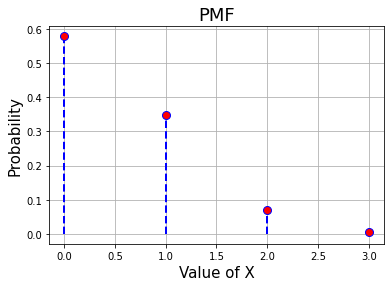
\includegraphics[width=\textwidth,height=5.5cm,keepaspectratio]{prv7.png}
		\caption{Probability Mass Function}
		\label{fig1}
	\end{figure}
    
\end{frame} 

\end{document}
